\documentclass[aspectratio=169]{beamer}
\usetheme{default}\usecolortheme{whale}
\usepackage{booktabs}\usepackage{amsmath}\usepackage{graphicx}\usepackage{tikz}
\definecolor{best}{RGB}{0,90,200}\newcommand{\bb}[1]{\textcolor{best}{\textbf{#1}}}
\definecolor{ok}{RGB}{0,140,60}\definecolor{wip}{RGB}{200,120,0}
\setbeamertemplate{navigation symbols}{}
\setbeamerfont{frametitle}{size=\large}
\title{Bitcoin Forecasting with VLA --- Meeting Update}\date{}
\begin{document}
\frame{\titlepage}
\begin{frame}{1. Recap --- previous meeting}
\large
\begin{itemize}
\item Previous \textbf{best model: v14\_groot\_1h} (DiT head, hourly, no normalisation).
\item All new experiments built on top of that baseline.
\end{itemize}
\vspace{1em}
\normalsize
\textbf{Key finding this round (preview):} v14's strong numbers turned out to be
\textbf{regime memorisation} (it rode the training-period uptrend), not real skill.
Target normalisation fixes this --- detailed in slide~4.
\end{frame}
\begin{frame}{Feedback from last meeting --- status}
\small
\begin{center}\begin{tabular}{lll}
\toprule
\# & Feedback & Status \\ \midrule
1 & Predict other coins (ETH, XRP) together & \textcolor{ok}{\textbf{Done}} (multi-asset) \\
2 & Predict bonds + S\&P simultaneously & \textcolor{ok}{\textbf{Done}} (macro exp.) \\
3 & Don't predict when markets closed & \textcolor{ok}{\textbf{Done}} (market-hours aligned) \\
4 & Make AER positive & \textcolor{wip}{\textbf{In progress}} (see slide 8) \\
5 & Try the RLDX-1 architecture & \textcolor{ok}{\textbf{Done}} (MSAT head) \\
6 & Check Kronos data contamination & \textcolor{ok}{\textbf{Done}} (June-2024 cutoff $\Rightarrow$ fold6 only) \\
\bottomrule
\end{tabular}\end{center}
\end{frame}
\begin{frame}{2. Trading strategies}
\small
\textbf{Signal:} from the predicted candles, expected move over horizon $k$: $\hat m=\hat p_{t+k}/p_t-1$. Trade if $|\hat m|>\theta$ (gate, $\theta\in\{0.1,0.3,0.5,1.0\}\%$).
\vspace{.6ex}
\begin{center}\begin{tabular}{ll}
\toprule
Strategy & Position rule \\ \midrule
\textbf{Long-only} & long if $\hat m>\theta$, else flat (never short) \\
\textbf{Long-short} & long if $\hat m>\theta$; short if $\hat m<-\theta$; else flat \\
\textbf{Magnitude} & size $=\mathrm{clip}(\hat m/s,-1,1)$ \\
\bottomrule
\end{tabular}\end{center}
\vspace{.4ex}
\footnotesize Metrics: ret (return), AER (excess vs B\&H), MDD. Slippage 0.1\%.
\end{frame}
\begin{frame}{How a trade works \& the $k$-slot backtest}
\small
\textbf{(1) Signal $\to$ enter $\to$ hold $k$ bars $\to$ exit.} At bar $t$ predict $k$ ahead; expected move $\hat m=\hat p_{t+k}/p_t-1$. Trade only if $|\hat m|>\theta$.
\begin{center}
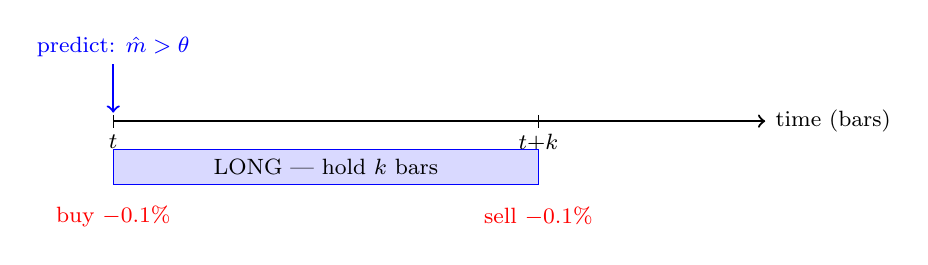
\begin{tikzpicture}[scale=0.9]
\draw[->,thick] (0,0)--(9.2,0) node[right]{\footnotesize time (bars)};
\foreach \x/\l in {0/{$t$},6/{$t{+}k$}} {\draw (\x,0.09)--(\x,-0.09); \node[below] at (\x,-0.05){\footnotesize \l};}
\node[align=center,blue] at (0,1.05){\footnotesize predict: $\hat m>\theta$};
\draw[->,thick,blue] (0,0.8)--(0,0.12);
\draw[fill=blue!15,draw=blue] (0,-0.9) rectangle (6,-0.4);
\node at (3,-0.65){\footnotesize LONG --- hold $k$ bars};
\node[red] at (0,-1.35){\footnotesize buy $-0.1\%$};
\node[red] at (6,-1.35){\footnotesize sell $-0.1\%$};
\end{tikzpicture}
\end{center}
\vspace{-0.5ex}
\textbf{(2) $k$-slot overlap.} A new signal every bar $\Rightarrow$ up to $k$ trades open at once. Capital is split into $k$ slots ($1/k$ each) so total exposure $\le100\%$ (no leverage from stride-1 overlap).
\begin{center}
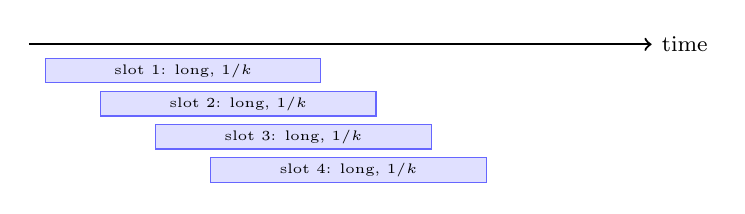
\begin{tikzpicture}[scale=0.7]
\draw[->,thick] (-0.3,0.7)--(11,0.7) node[right]{\footnotesize time};
\foreach \i/\n in {0/1,1/2,2/3,3/4}{
  \draw[fill=blue!12,draw=blue!60] (\i, -\i*0.6) rectangle (\i+5,-\i*0.6+0.45);
  \node[font=\tiny] at (\i+2.5,-\i*0.6+0.22){slot \n: long, $1/k$};
}
\end{tikzpicture}
\end{center}
\vspace{-0.5ex}
\footnotesize Combined equity curve $\to$ ret (principal return), AER (excess vs B\&H), MDD.
\end{frame}
\begin{frame}{3. This round --- experiment design (4 axes)}
\small
Every experiment is a combination of \textbf{4 independent choices}:
\begin{center}\begin{tabular}{lll}
\toprule
Axis & Options & What it tests \\ \midrule
\textbf{Head} & DiT / \textbf{MSAT} & cross-attn vs joint-attn (RLDX-1) \\
\textbf{Assets} & BTC / BTC+ETH+XRP & does multi-asset help? \\
\textbf{Diffusion scope} & all-diff / read-off & generate all vs BTC-only+aux \\
\textbf{Normalisation} & on / off & target $\div$std (scale to noise) \\
\bottomrule
\end{tabular}\end{center}
\vspace{.6ex}
\footnotesize \textbf{MSAT} (from RLDX-1) = multi-stream joint self-attention over VL + action tokens
(vs DiT's single-stream cross-attention). VLM (Qwen3-VL) frozen; only the action head trains.
Walk-forward 6-fold (2020--2025), BTC-only metrics, 0.1\% slippage.
\end{frame}
\begin{frame}{4. Why normalisation? --- per-fold long-ratio ($k=6$)}
\small Fraction long in each fold. \textbf{Raw (no-norm) swings to extremes} (all-long$\approx$1 / all-short$\approx$0) = memorising each fold's trend. Normalisation keeps it moderate.\\[.5ex]
\begin{center}\resizebox{\ifdim\width>\linewidth\linewidth\else\width\fi}{!}{\begin{tabular}{lccccccc}\toprule
Experiment & F1 & F2 & F3 & F4 & F5 & F6 & $\sigma$ \\ \midrule
DiT-Multi-RO-raw & 1.00 & 0.18 & 0.44 & 0.75 & 0.92 & 0.12 & \textbf{0.343} \\
DiT-BTC & 0.71 & 0.39 & 0.29 & 0.58 & 0.72 & 0.30 & \bb{0.178} \\
DiT-Multi & 0.83 & 0.41 & 0.48 & 0.72 & 0.68 & 0.57 & \bb{0.142} \\
MSAT-BTC & 0.74 & 0.46 & 0.45 & 0.58 & 0.60 & 0.52 & \bb{0.097} \\
MSAT-Multi & 0.73 & 0.43 & 0.46 & 0.57 & 0.60 & 0.42 & \bb{0.111} \\
MSAT-Multi-RO-raw & 1.00 & 0.06 & 0.00 & 0.15 & 1.00 & 0.19 & \textbf{0.428} \\
MSAT-Multi-raw & 0.97 & 0.01 & 0.01 & 0.88 & 0.87 & 0.40 & \textbf{0.406} \\
MSAT-Multi-RO & 0.56 & 0.42 & 0.39 & 0.48 & 0.43 & 0.57 & \bb{0.068} \\
\bottomrule\end{tabular}}\end{center}
\footnotesize $\sigma$=across-fold std (regime index). Raw exps reach 0.00 \& 1.00; normalised stay $\approx$0.3--0.7. \textbf{Normalisation cuts $\sigma$ by $\sim$3$\times$ and does NOT sacrifice real return} (raw's higher return is fold-1 bull memorisation).\end{frame}
\begin{frame}{4b. Diffusion scope --- all-diffusion vs read-off}
\small
For multi-asset: how are ETH/XRP handled alongside BTC?
\vspace{.6ex}
\begin{center}\begin{tabular}{ll}
\toprule
\textbf{all-diffusion} & all 3 assets generated jointly by diffusion (one 12-dim vector) \\
\textbf{read-off (RO)} & \textbf{BTC only} by diffusion; ETH/XRP via a small MLP (L1 aux) \\
\bottomrule
\end{tabular}\end{center}
\vspace{.8ex}
\begin{columns}
\column{0.5\textwidth}
\centering \footnotesize \textbf{all-diffusion}\\[.5ex]
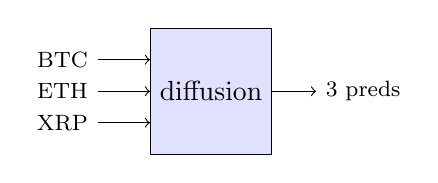
\begin{tikzpicture}[scale=0.8]
\node[draw,fill=blue!12,minimum width=1.5cm,minimum height=1.6cm] (d) at (2,0){diffusion};
\foreach \y/\a in {0.5/BTC,0/ETH,-0.5/XRP}{\draw[->] (0.2,\y) node[left]{\footnotesize \a} -- (d.west|-0,\y);}
\draw[->] (d.east) -- ++(0.7,0) node[right]{\footnotesize 3 preds};
\end{tikzpicture}
\column{0.5\textwidth}
\centering \footnotesize \textbf{read-off}\\[.5ex]
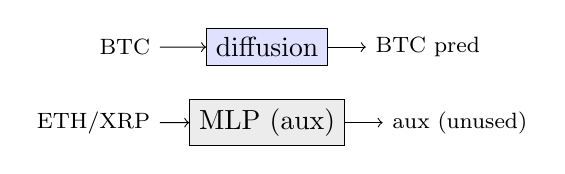
\begin{tikzpicture}[scale=0.8]
\node[draw,fill=blue!12,minimum width=1.3cm] (d) at (2,0.6){diffusion};
\node[draw,fill=gray!15,minimum width=1.3cm] (m) at (2,-0.6){MLP (aux)};
\draw[->] (0.3,0.6) node[left]{\footnotesize BTC} -- (d.west);
\draw[->] (d.east) -- ++(0.6,0) node[right]{\footnotesize BTC pred};
\draw[->] (0.3,-0.6) node[left]{\footnotesize ETH/XRP} -- (m.west);
\draw[->] (m.east) -- ++(0.6,0) node[right]{\footnotesize aux (unused)};
\end{tikzpicture}
\end{columns}
\vspace{.6ex}
\footnotesize \textbf{Read-off} = ETH/XRP as an auxiliary regularizer to help BTC's representation; \emph{not used at inference}. \textbf{Result:} under normalisation, all-diffusion is slightly better --- the dominant factor is normalisation, not diffusion scope.
\end{frame}

\begin{frame}{5. Experiments run this round}
\small\begin{center}\begin{tabular}{lllll}\toprule
Experiment & Head & Assets & Diff-scope & Norm \\ \midrule
DiT-Multi-RO-raw & DiT & BTC+ETH+XRP & read-off$^\dagger$ & \textbf{off} \\
DiT-BTC & DiT & BTC & --- & on \\
DiT-Multi & DiT & BTC+ETH+XRP & all-diff & on \\
MSAT-BTC & \textbf{MSAT} & BTC & --- & on \\
MSAT-Multi & \textbf{MSAT} & BTC+ETH+XRP & all-diff & on \\
MSAT-Multi-RO-raw & \textbf{MSAT} & BTC+ETH+XRP & read-off$^\dagger$ & \textbf{off} \\
MSAT-Multi-raw & \textbf{MSAT} & BTC+ETH+XRP & all-diff & \textbf{off} \\
MSAT-Multi-RO & \textbf{MSAT} & BTC+ETH+XRP & read-off$^\dagger$ & on \\
\midrule Kronos & pretrained & BTC & --- & --- \\
macro ($\times$4) & DiT & BTC+S\&P/bonds & all-diff & on \\
\bottomrule\end{tabular}\end{center}
\footnotesize 8 crypto experiments = full 4-axis coverage. $^\dagger$read-off = ETH/XRP as auxiliary regression (see slide 4b). + Kronos + 4 macro.\end{frame}
\begin{frame}{6. Per-experiment DA \& Long\_ns (6-fold avg)}
\scriptsize\textbf{Directional Accuracy}\\[.2ex]
\begin{center}\resizebox{\ifdim\width>\linewidth\linewidth\else\width\fi}{!}{\begin{tabular}{lcccc}\toprule
Experiment & $k=1$ & $k=3$ & $k=6$ & $k=12$ \\ \midrule
DiT-Multi-RO-raw & 0.509 & 0.517 & \bb{0.527} & 0.525 \\
DiT-BTC & 0.507 & 0.511 & 0.517 & 0.517 \\
DiT-Multi & 0.505 & 0.515 & 0.512 & 0.515 \\
MSAT-BTC & 0.511 & \bb{0.517} & 0.507 & 0.522 \\
MSAT-Multi & 0.502 & 0.511 & 0.513 & 0.506 \\
MSAT-Multi-RO-raw & \bb{0.516} & 0.516 & 0.512 & \bb{0.532} \\
MSAT-Multi-raw & 0.511 & 0.513 & 0.523 & 0.527 \\
MSAT-Multi-RO & 0.498 & 0.487 & 0.504 & 0.491 \\
\bottomrule\end{tabular}}\end{center}
\vspace{.2ex}\scriptsize\textbf{Long\_ns} (long-ratio, no-slippage; near 1 = always-long)\\[.2ex]
\begin{center}\resizebox{\ifdim\width>\linewidth\linewidth\else\width\fi}{!}{\begin{tabular}{lcccc}\toprule
Experiment & $k=1$ & $k=3$ & $k=6$ & $k=12$ \\ \midrule
DiT-Multi-RO-raw & 0.56 & 0.58 & 0.57 & 0.57 \\
DiT-BTC & 0.52 & 0.52 & 0.50 & 0.49 \\
DiT-Multi & 0.56 & 0.59 & 0.62 & 0.65 \\
MSAT-BTC & 0.52 & 0.55 & 0.56 & 0.58 \\
MSAT-Multi & 0.53 & 0.52 & 0.54 & 0.55 \\
MSAT-Multi-RO-raw & 0.48 & 0.44 & 0.40 & 0.36 \\
MSAT-Multi-raw & 0.47 & 0.51 & 0.52 & 0.55 \\
MSAT-Multi-RO & 0.49 & 0.49 & 0.48 & 0.45 \\
\bottomrule\end{tabular}}\end{center}
\footnotesize DA barely above 0.5 (weak signal); Long\_ns spread across folds = regime bias (next slide).\end{frame}
\begin{frame}{7. Long-only strategy, $\theta=0.1\%$ --- ret / AER (6-fold avg)}
\small each cell = \textbf{ret / AER}\\[.4ex]
\begin{center}\resizebox{\ifdim\width>\linewidth\linewidth\else\width\fi}{!}{\begin{tabular}{lcccc}\toprule
Experiment & $k=1$ & $k=3$ & $k=6$ & $k=12$ \\ \midrule
DiT-Multi-RO-raw & -0.264/-0.336 & -0.054/-0.124 & \bb{+0.033/-0.039} & +0.046/-0.024 \\
DiT-BTC & \bb{-0.161/-0.233} & -0.042/-0.112 & +0.023/-0.049 & +0.037/-0.033 \\
DiT-Multi & -0.226/-0.297 & -0.078/-0.148 & -0.013/-0.085 & +0.024/-0.046 \\
MSAT-BTC & -0.193/-0.264 & -0.061/-0.130 & -0.007/-0.079 & +0.039/-0.032 \\
MSAT-Multi & -0.205/-0.277 & -0.043/-0.113 & +0.016/-0.056 & +0.026/-0.044 \\
MSAT-Multi-RO-raw & -0.184/-0.255 & \bb{-0.028/-0.098} & +0.026/-0.046 & \bb{+0.057/-0.013} \\
MSAT-Multi-raw & -0.199/-0.270 & -0.047/-0.117 & +0.011/-0.061 & +0.047/-0.023 \\
MSAT-Multi-RO & -0.176/-0.248 & -0.050/-0.120 & -0.003/-0.075 & -0.002/-0.072 \\
\bottomrule\end{tabular}}\end{center}
\footnotesize ret=principal return, AER=excess vs B\&H. B\&H(6-fold)$\approx+7.2\%$.\end{frame}
\begin{frame}{7. Long-only strategy, $\theta=0.3\%$ --- ret / AER (6-fold avg)}
\small each cell = \textbf{ret / AER}\\[.4ex]
\begin{center}\resizebox{\ifdim\width>\linewidth\linewidth\else\width\fi}{!}{\begin{tabular}{lcccc}\toprule
Experiment & $k=1$ & $k=3$ & $k=6$ & $k=12$ \\ \midrule
DiT-Multi-RO-raw & -0.249/-0.321 & -0.053/-0.123 & \bb{+0.037/-0.035} & +0.048/-0.022 \\
DiT-BTC & -0.076/-0.147 & \bb{-0.005/-0.075} & +0.026/-0.046 & +0.038/-0.033 \\
DiT-Multi & -0.106/-0.178 & -0.074/-0.144 & -0.016/-0.088 & +0.028/-0.042 \\
MSAT-BTC & -0.104/-0.176 & -0.055/-0.125 & +0.003/-0.069 & +0.034/-0.036 \\
MSAT-Multi & -0.074/-0.145 & -0.041/-0.111 & +0.022/-0.050 & +0.026/-0.044 \\
MSAT-Multi-RO-raw & -0.156/-0.228 & -0.017/-0.087 & +0.030/-0.042 & \bb{+0.058/-0.012} \\
MSAT-Multi-raw & -0.134/-0.205 & -0.039/-0.109 & +0.014/-0.059 & +0.049/-0.022 \\
MSAT-Multi-RO & \bb{-0.050/-0.121} & -0.042/-0.112 & -0.009/-0.081 & +0.003/-0.067 \\
\bottomrule\end{tabular}}\end{center}
\footnotesize ret=principal return, AER=excess vs B\&H. B\&H(6-fold)$\approx+7.2\%$.\end{frame}
\begin{frame}{7. Long-only strategy, $\theta=0.5\%$ --- ret / AER (6-fold avg)}
\small each cell = \textbf{ret / AER}\\[.4ex]
\begin{center}\resizebox{\ifdim\width>\linewidth\linewidth\else\width\fi}{!}{\begin{tabular}{lcccc}\toprule
Experiment & $k=1$ & $k=3$ & $k=6$ & $k=12$ \\ \midrule
DiT-Multi-RO-raw & -0.230/-0.301 & -0.047/-0.117 & +0.035/-0.037 & +0.049/-0.022 \\
DiT-BTC & \bb{-0.033/-0.104} & \bb{+0.011/-0.059} & \bb{+0.040/-0.032} & +0.035/-0.035 \\
DiT-Multi & -0.053/-0.124 & -0.046/-0.116 & -0.026/-0.098 & +0.031/-0.039 \\
MSAT-BTC & -0.052/-0.123 & -0.043/-0.113 & +0.013/-0.059 & +0.035/-0.035 \\
MSAT-Multi & -0.045/-0.116 & -0.017/-0.087 & +0.027/-0.045 & +0.028/-0.042 \\
MSAT-Multi-RO-raw & -0.139/-0.210 & -0.014/-0.084 & +0.030/-0.042 & \bb{+0.059/-0.012} \\
MSAT-Multi-raw & -0.101/-0.172 & -0.035/-0.105 & +0.014/-0.058 & +0.049/-0.021 \\
MSAT-Multi-RO & -0.044/-0.116 & -0.031/-0.101 & -0.008/-0.080 & +0.004/-0.066 \\
\bottomrule\end{tabular}}\end{center}
\footnotesize ret=principal return, AER=excess vs B\&H. B\&H(6-fold)$\approx+7.2\%$.\end{frame}
\begin{frame}{7. Long-only strategy, $\theta=1.0\%$ --- ret / AER (6-fold avg)}
\small each cell = \textbf{ret / AER}\\[.4ex]
\begin{center}\resizebox{\ifdim\width>\linewidth\linewidth\else\width\fi}{!}{\begin{tabular}{lcccc}\toprule
Experiment & $k=1$ & $k=3$ & $k=6$ & $k=12$ \\ \midrule
DiT-Multi-RO-raw & -0.165/-0.236 & -0.035/-0.105 & \bb{+0.035/-0.037} & +0.050/-0.020 \\
DiT-BTC & \bb{-0.003/-0.075} & \bb{+0.007/-0.063} & +0.026/-0.046 & +0.030/-0.040 \\
DiT-Multi & -0.005/-0.076 & -0.017/-0.086 & -0.014/-0.086 & +0.024/-0.047 \\
MSAT-BTC & -0.024/-0.095 & -0.014/-0.083 & +0.013/-0.059 & +0.036/-0.035 \\
MSAT-Multi & -0.006/-0.078 & -0.003/-0.073 & +0.015/-0.057 & +0.029/-0.042 \\
MSAT-Multi-RO-raw & -0.125/-0.197 & -0.011/-0.081 & +0.034/-0.038 & \bb{+0.059/-0.011} \\
MSAT-Multi-raw & -0.025/-0.097 & -0.025/-0.095 & +0.016/-0.056 & +0.050/-0.021 \\
MSAT-Multi-RO & -0.010/-0.081 & -0.006/-0.075 & -0.004/-0.076 & +0.006/-0.064 \\
\bottomrule\end{tabular}}\end{center}
\footnotesize ret=principal return, AER=excess vs B\&H. B\&H(6-fold)$\approx+7.2\%$.\end{frame}
\begin{frame}{7. Long-short strategy, $\theta=0.1\%$ --- ret / AER (6-fold avg)}
\small each cell = \textbf{ret / AER}\\[.4ex]
\begin{center}\resizebox{\ifdim\width>\linewidth\linewidth\else\width\fi}{!}{\begin{tabular}{lcccc}\toprule
Experiment & $k=1$ & $k=3$ & $k=6$ & $k=12$ \\ \midrule
DiT-Multi-RO-raw & -0.438/-0.509 & \bb{-0.127/-0.197} & \bb{+0.007/-0.065} & +0.026/-0.045 \\
DiT-BTC & \bb{-0.323/-0.394} & -0.139/-0.209 & -0.031/-0.103 & +0.003/-0.067 \\
DiT-Multi & -0.376/-0.447 & -0.162/-0.232 & -0.057/-0.129 & -0.003/-0.074 \\
MSAT-BTC & -0.339/-0.410 & -0.144/-0.214 & -0.057/-0.129 & +0.014/-0.057 \\
MSAT-Multi & -0.365/-0.436 & -0.130/-0.200 & -0.026/-0.098 & -0.011/-0.082 \\
MSAT-Multi-RO-raw & -0.383/-0.455 & -0.132/-0.202 & -0.041/-0.113 & +0.027/-0.043 \\
MSAT-Multi-raw & -0.428/-0.499 & -0.146/-0.216 & -0.040/-0.112 & \bb{+0.032/-0.038} \\
MSAT-Multi-RO & -0.373/-0.445 & -0.168/-0.238 & -0.072/-0.144 & -0.065/-0.136 \\
\bottomrule\end{tabular}}\end{center}
\footnotesize ret=principal return, AER=excess vs B\&H. B\&H(6-fold)$\approx+7.2\%$.\end{frame}
\begin{frame}{7. Long-short strategy, $\theta=0.3\%$ --- ret / AER (6-fold avg)}
\small each cell = \textbf{ret / AER}\\[.4ex]
\begin{center}\resizebox{\ifdim\width>\linewidth\linewidth\else\width\fi}{!}{\begin{tabular}{lcccc}\toprule
Experiment & $k=1$ & $k=3$ & $k=6$ & $k=12$ \\ \midrule
DiT-Multi-RO-raw & -0.412/-0.483 & -0.121/-0.191 & \bb{+0.011/-0.061} & +0.029/-0.042 \\
DiT-BTC & -0.180/-0.252 & \bb{-0.076/-0.146} & -0.008/-0.080 & +0.016/-0.055 \\
DiT-Multi & -0.171/-0.242 & -0.127/-0.197 & -0.050/-0.122 & +0.005/-0.065 \\
MSAT-BTC & -0.167/-0.239 & -0.109/-0.179 & -0.034/-0.106 & +0.013/-0.057 \\
MSAT-Multi & \bb{-0.144/-0.215} & -0.100/-0.170 & -0.002/-0.074 & -0.004/-0.074 \\
MSAT-Multi-RO-raw & -0.318/-0.389 & -0.107/-0.177 & -0.036/-0.108 & +0.027/-0.043 \\
MSAT-Multi-raw & -0.302/-0.373 & -0.117/-0.187 & -0.028/-0.100 & \bb{+0.034/-0.037} \\
MSAT-Multi-RO & -0.170/-0.242 & -0.129/-0.199 & -0.074/-0.146 & -0.047/-0.117 \\
\bottomrule\end{tabular}}\end{center}
\footnotesize ret=principal return, AER=excess vs B\&H. B\&H(6-fold)$\approx+7.2\%$.\end{frame}
\begin{frame}{7. Long-short strategy, $\theta=0.5\%$ --- ret / AER (6-fold avg)}
\small each cell = \textbf{ret / AER}\\[.4ex]
\begin{center}\resizebox{\ifdim\width>\linewidth\linewidth\else\width\fi}{!}{\begin{tabular}{lcccc}\toprule
Experiment & $k=1$ & $k=3$ & $k=6$ & $k=12$ \\ \midrule
DiT-Multi-RO-raw & -0.384/-0.456 & -0.108/-0.178 & +0.008/-0.064 & +0.027/-0.043 \\
DiT-BTC & -0.098/-0.169 & \bb{-0.031/-0.101} & \bb{+0.013/-0.059} & +0.021/-0.050 \\
DiT-Multi & -0.082/-0.153 & -0.085/-0.155 & -0.053/-0.125 & +0.008/-0.062 \\
MSAT-BTC & -0.096/-0.167 & -0.066/-0.136 & -0.010/-0.082 & +0.019/-0.051 \\
MSAT-Multi & \bb{-0.053/-0.125} & -0.044/-0.114 & +0.004/-0.068 & +0.006/-0.064 \\
MSAT-Multi-RO-raw & -0.277/-0.348 & -0.092/-0.162 & -0.023/-0.095 & +0.028/-0.042 \\
MSAT-Multi-raw & -0.223/-0.294 & -0.100/-0.170 & -0.028/-0.100 & \bb{+0.035/-0.036} \\
MSAT-Multi-RO & -0.115/-0.186 & -0.099/-0.169 & -0.063/-0.135 & -0.036/-0.106 \\
\bottomrule\end{tabular}}\end{center}
\footnotesize ret=principal return, AER=excess vs B\&H. B\&H(6-fold)$\approx+7.2\%$.\end{frame}
\begin{frame}{7. Long-short strategy, $\theta=1.0\%$ --- ret / AER (6-fold avg)}
\small each cell = \textbf{ret / AER}\\[.4ex]
\begin{center}\resizebox{\ifdim\width>\linewidth\linewidth\else\width\fi}{!}{\begin{tabular}{lcccc}\toprule
Experiment & $k=1$ & $k=3$ & $k=6$ & $k=12$ \\ \midrule
DiT-Multi-RO-raw & -0.280/-0.352 & -0.094/-0.164 & +0.005/-0.067 & +0.031/-0.040 \\
DiT-BTC & -0.021/-0.093 & -0.017/-0.087 & \bb{+0.007/-0.065} & +0.021/-0.050 \\
DiT-Multi & -0.013/-0.085 & -0.038/-0.108 & -0.020/-0.092 & +0.016/-0.054 \\
MSAT-BTC & -0.033/-0.104 & -0.026/-0.096 & -0.002/-0.074 & +0.024/-0.046 \\
MSAT-Multi & \bb{-0.004/-0.076} & \bb{-0.007/-0.077} & +0.007/-0.065 & +0.017/-0.054 \\
MSAT-Multi-RO-raw & -0.201/-0.272 & -0.085/-0.155 & -0.010/-0.082 & \bb{+0.038/-0.032} \\
MSAT-Multi-raw & -0.089/-0.160 & -0.057/-0.127 & -0.014/-0.086 & +0.037/-0.033 \\
MSAT-Multi-RO & -0.022/-0.093 & -0.026/-0.096 & -0.042/-0.114 & -0.026/-0.096 \\
\bottomrule\end{tabular}}\end{center}
\footnotesize ret=principal return, AER=excess vs B\&H. B\&H(6-fold)$\approx+7.2\%$.\end{frame}
\begin{frame}{8. Best strategy per experiment (6-fold avg) \& AER status}
\small Highest-ret setup per experiment (over all strategies/$\theta$/$k$):\\[.4ex]
\begin{center}\resizebox{\ifdim\width>\linewidth\linewidth\else\width\fi}{!}{\begin{tabular}{llccc}\toprule
Experiment & Strategy & $k$ & ret & AER \\ \midrule
DiT-Multi-RO-raw & long-only $\theta1.0$ & 12 & +0.050 & -0.020 \\
DiT-BTC & long-only $\theta0.5$ & 6 & +0.040 & -0.032 \\
DiT-Multi & long-only $\theta0.5$ & 12 & +0.031 & -0.039 \\
MSAT-BTC & long-only $\theta0.1$ & 12 & +0.039 & -0.032 \\
MSAT-Multi & long-only $\theta1.0$ & 12 & +0.029 & -0.042 \\
MSAT-Multi-RO-raw & long-only $\theta1.0$ & 12 & \bb{+0.059} & -0.011 \\
MSAT-Multi-raw & long-only $\theta1.0$ & 12 & +0.050 & -0.021 \\
MSAT-Multi-RO & long-only $\theta1.0$ & 12 & +0.006 & -0.064 \\
\bottomrule\end{tabular}}\end{center}
\vspace{.3ex}\footnotesize \textbf{AER status:} \textcolor{wip}{on 6-fold average NO setup has ret$>$0 \emph{and} AER$>$0} (can't beat B\&H's $+7.2\%$). On fold6 (down market) a few do. \textbf{New trend/downside strategies being tested to fix this.}\end{frame}
\begin{frame}{8b. B\&H is skewed by fold1 (2020) --- AER on fold2--6}
\small \textbf{B\&H per-fold return} (each fold = that year's December):\\[.3ex]
\begin{center}\footnotesize\begin{tabular}{lccccccc}\toprule
& F1(20) & F2(21) & F3(22) & F4(23) & F5(24) & F6(25) & \textbf{avg} \\ \midrule
B\&H $k{=}6$ & \bb{+0.492} & +0.012 & -0.023 & +0.021 & -0.016 & -0.053 & +0.072 \\
\bottomrule\end{tabular}\end{center}
\footnotesize \textbf{fold1(2020) alone is $+49\%$}; the average $+7.2\%$ is almost entirely this one bull month. fold2--6 B\&H is actually $-1.2\%$.\\[.8ex]
\small \textbf{On the representative fold2--6 average, some setups now beat B\&H (AER$>$0 \emph{and} ret$>$0):}\\[.3ex]
\begin{center}\footnotesize\begin{tabular}{lllcc}\toprule
Experiment & Strategy & $k$ & ret & AER \\ \midrule
\bb{MSAT-BTC} & long-only $\theta1.0$ & 12 & \bb{+0.001} & \bb{+0.019} \\
\bb{MSAT-Multi} & long-only $\theta1.0$ & 6 & \bb{+0.003} & \bb{+0.014} \\
\bottomrule\end{tabular}\end{center}
\footnotesize Both are \textbf{normalised MSAT} models at high gate ($\theta1.0\%$). Caveat: absolute ret still $\approx0$; excludes fold1 as an outlier (defensible: $+49\%$ distorts the mean).\end{frame}
\begin{frame}{8c. AER$>$0 setups --- per-fold breakdown}
\small Both AER$>$0 setups: only fold1 (2020 bull) loses to B\&H; \textbf{folds 2--6 mostly beat it}.\\[.5ex]
\begin{center}\footnotesize\begin{tabular}{lccccccc}\toprule
\textbf{MSAT-BTC} LO$\theta1.0$ $k12$ & F1(20) & F2(21) & F3(22) & F4(23) & F5(24) & F6(25) & avg2--6 \\ \midrule
\quad ret & +0.208 & +0.003 & +0.001 & +0.029 & +0.001 & -0.028 & +0.001 \\
\quad AER & -0.301 & \bb{+0.017} & \bb{+0.026} & \bb{+0.008} & \bb{+0.019} & \bb{+0.024} & \bb{+0.019} \\
\bottomrule\end{tabular}\end{center}
\vspace{.3ex}\begin{center}\footnotesize\begin{tabular}{lccccccc}\toprule
\textbf{MSAT-Multi} LO$\theta1.0$ $k6$ & F1(20) & F2(21) & F3(22) & F4(23) & F5(24) & F6(25) & avg2--6 \\ \midrule
\quad ret & +0.077 & +0.036 & -0.007 & -0.006 & -0.005 & -0.004 & +0.003 \\
\quad AER & -0.415 & \bb{+0.024} & \bb{+0.016} & -0.027 & \bb{+0.010} & \bb{+0.049} & \bb{+0.014} \\
\midrule B\&H ret & +0.492 & +0.012 & -0.023 & +0.021 & -0.016 & -0.053 & \\
\bottomrule\end{tabular}\end{center}
\footnotesize Blue = AER$>$0 (beats B\&H). Excluding fold1, MSAT-BTC wins 5/5 folds, MSAT-Multi 4/5. fold6 (down market): strong defence (AER $+2$--$5\%$). Absolute ret $\approx0$ (bearish 2021--25).\end{frame}
\begin{frame}{9. Comparison with Kronos (fold6 only, clean OOS)}
\small Kronos (June-2024 cutoff) is valid only on fold6 (2025). Best-strategy \textbf{ret / AER} on fold6:\\[.4ex]
\begin{center}\resizebox{\ifdim\width>\linewidth\linewidth\else\width\fi}{!}{\begin{tabular}{lcccc}\toprule
Model & $k=1$ & $k=3$ & $k=6$ & $k=12$ \\ \midrule
DiT-Multi-RO-raw & -0.099/-0.049 & -0.059/-0.010 & -0.024/+0.030 & -0.010/+0.042 \\
DiT-BTC & +0.013/+0.062 & +0.011/+0.060 & -0.014/+0.039 & +0.003/+0.055 \\
DiT-Multi & -0.004/+0.045 & +0.014/+0.064 & -0.036/+0.018 & -0.043/+0.009 \\
MSAT-BTC & -0.004/+0.046 & -0.070/-0.020 & -0.011/+0.043 & -0.028/+0.024 \\
MSAT-Multi & +0.004/+0.053 & +0.010/+0.060 & -0.004/+0.049 & +0.004/+0.056 \\
MSAT-Multi-RO-raw & -0.110/-0.060 & -0.028/+0.021 & -0.028/+0.025 & -0.003/+0.049 \\
MSAT-Multi-raw & \bb{+0.014/+0.064} & -0.010/+0.040 & -0.007/+0.047 & +0.020/+0.072 \\
MSAT-Multi-RO & -0.009/+0.041 & +0.018/+0.067 & -0.026/+0.027 & -0.011/+0.041 \\
\bb{Kronos} & +0.002/+0.051 & \bb{+0.036/+0.086} & \bb{+0.059/+0.112} & \bb{+0.125/+0.178} \\
\midrule B\&H ret & -0.050 & -0.049 & -0.053 & -0.052 \\
\bottomrule\end{tabular}}\end{center}
\footnotesize Our models trained on 2025 Jan--Oct; Kronos never saw 2025. Yet \textbf{only Kronos is positive on fold6}, widening with $k$ --- pretrained foundation model generalises better.\end{frame}
\begin{frame}{10. Macro experiments (BTC + S\&P/bonds) --- ret / AER}
\small Market-hours-aligned dataset, \textbf{2-fold (2024, 2025)}, predicts only when US markets open. each cell = \textbf{ret / AER} (2-fold avg)\\[.5ex]
\begin{center}\resizebox{\ifdim\width>\linewidth\linewidth\else\width\fi}{!}{\begin{tabular}{lcccc}\toprule
Experiment & $k=1$ & $k=3$ & $k=6$ & $k=12$ \\ \midrule
baseline (BTC only) & \bb{-0.020/+0.043} & -0.034/+0.022 & \bb{-0.027/+0.028} & \bb{-0.022/+0.023} \\
BTC+SPY+TLT (20yr+) & -0.146/-0.084 & -0.037/+0.019 & -0.029/+0.026 & -0.049/-0.004 \\
BTC+SPY+IEF (7--10yr) & -0.090/-0.027 & -0.055/+0.001 & -0.051/+0.005 & -0.044/+0.001 \\
BTC+SPY+SHY (1--3yr) & -0.032/+0.031 & \bb{-0.011/+0.046} & -0.047/+0.008 & -0.039/+0.006 \\
\midrule B\&H ret & -0.062 & -0.056 & -0.055 & -0.045 \\
\bottomrule\end{tabular}}\end{center}
\footnotesize ret=portfolio return, AER=excess vs B\&H. \textbf{Adding S\&P/bonds does not improve BTC} (baseline is best/tied at most $k$; consistent across all $k$). AER positive because macro B\&H $<0$ (down market). TLT/IEF/SHY = long/mid/short-term US Treasuries (20yr+/7--10yr/1--3yr); feedback \#3 (market-hours) via timestamp intersection.\end{frame}
\begin{frame}{11. Conclusions}
\small
\begin{enumerate}
\item \textbf{Normalisation is the key win}: cuts regime bias $\sigma$ $\sim$3$\times$; raw v14's high return was uptrend memorisation (worst on clean fold6).
\item \textbf{Multi-asset helps only with MSAT} (joint attention captures cross-asset structure); it hurts under DiT.
\item \textbf{MSAT vs DiT}: MSAT wins for multi-asset, DiT wins for single-asset / read-off.
\item \textbf{read-off vs all-diffusion}: under normalisation, all-diffusion is slightly better.
\item \textbf{No model beats B\&H} (+7.2\%) on 6-fold average; \textbf{AER$>$0 only on fold6}.
\item \textbf{On clean OOS (fold6) only Kronos is positive} --- foundation model $>$ from-scratch.
\end{enumerate}
\vspace{.3ex}
\textbf{Best of ours: v15\_btc / v16\_msat} (normalised). Next: input normalisation + risk-managed strategies (trend/downside) for AER$>$0.
\end{frame}
\end{document}